%%
%% This is file `sample-sigconf.tex',
%% generated with the docstrip utility.
%%
%% The original source files were:
%%
%% samples.dtx  (with options: `sigconf')
%% 
%% IMPORTANT NOTICE:
%% 
%% For the copyright see the source file.
%% 
%% Any modified versions of this file must be renamed
%% with new filenames distinct from sample-sigconf.tex.
%% 
%% For distribution of the original source see the terms
%% for copying and modification in the file samples.dtx.
%% 
%% This generated file may be distributed as long as the
%% original source files, as listed above, are part of the
%% same distribution. (The sources need not necessarily be
%% in the same archive or directory.)
%%
%% The first command in your LaTeX source must be the \documentclass command.
\documentclass[sigconf, anonymous, review]{acmart}
\usepackage{multirow}

%%
%% \BibTeX command to typeset BibTeX logo in the docs
\AtBeginDocument{%
  \providecommand\BibTeX{{%
    \normalfont B\kern-0.5em{\scshape i\kern-0.25em b}\kern-0.8em\TeX}}}


%% Rights management information.  This information is sent to you
%% when you complete the rights form.  These commands have SAMPLE
%% values in them; it is your responsibility as an author to replace
%% the commands and values with those provided to you when you
%% complete the rights form.
%\setcopyright{acmcopyright}
%\copyrightyear{2018}
%\acmYear{2018}
%\acmDOI{10.1145/1122445.1122456}

%% These commands are for a PROCEEDINGS abstract or paper.
%\acmConference[Woodstock '18]{Woodstock '18: ACM Symposium on Neural
%  Gaze Detection}{June 03--05, 2018}{Woodstock, NY}
%\acmBooktitle{Woodstock '18: ACM Symposium on Neural Gaze Detection,
%  June 03--05, 2018, Woodstock, NY}
%\acmPrice{15.00}
%\acmISBN{978-1-4503-XXXX-X/18/06}


%%
%% Submission ID.
%% Use this when submitting an article to a sponsored event. You'll
%% receive a unique submission ID from the organizers
%% of the event, and this ID should be used as the parameter to this command.
%%\acmSubmissionID{123-A56-BU3}

%%
%% The majority of ACM publications use numbered citations and
%% references.  The command \citestyle{authoryear} switches to the
%% "author year" style.
%%
%% If you are preparing content for an event
%% sponsored by ACM SIGGRAPH, you must use the "author year" style of
%% citations and references.
%% Uncommenting
%% the next command will enable that style.
%%\citestyle{acmauthoryear}

%\usepackage{libertine}

\usepackage{booktabs}
\usepackage{subfigure}
\usepackage{xspace}
%%\usepackage{amsmath}
\usepackage{epstopdf} 
\usepackage{algorithm}
\usepackage{url}
%%\usepackage{algorithmicx} 
\usepackage{algpseudocode}
%%\usepackage{color}
\usepackage{ulem}

\newcommand{\comments}[2]{{\bf[\textcolor{blue}{#1}: \textcolor{red}{#2}]}}

%\newcommand{\codecomment}[1] {\emph{\small{//#1}}}
\newcommand{\codecomment}[1] {\textit{\small{//#1}}}
\newcommand{\codelinecomment}[1]{\textit{\small{/* #1 */}}}

\newcommand{\codepink}[1]{\textcolor{magenta}{#1}}
\newcommand{\codeblue}[1]{\textcolor{blue}{#1}}

\newcommand{\green}[1]{\textcolor{black}{#1}}
\newcommand{\blue}[1]{\textcolor{blue}{#1}}
\newcommand{\red}[1]{\textcolor{red}{\sout{#1}}}
\newcommand{\pink}[1]{\textcolor{purple}{#1}}
\newcommand{\hlight}[1]{\textcolor{purple}{#1}}
\newcommand{\zcl}[1]{\comments{Chuanlei}{#1}}
\newcommand{\zwh}[1]{{\comments{Weihua}{#1}}}
\newcommand{\lyz}[1]{{\comments{LYZ}{#1}}}
\newcommand{\lp}[1]{{\comments{LPeng}{#1}}}


\newcommand{\btree} {B+tree\xspace}
\newcommand{\txtree}{STM-based GPU \btree\xspace}
\newcommand{\base}{STM-based GPU B+tree\xspace}
\newcommand{\baseshort}{STM GB-tree\xspace}
\newcommand{\locktree}{lock-baed GB-tree\xspace}
\newcommand{\ucdavis}{lock-based GPU B-tree\xspace}
\newcommand{\ucdavisshort}{Lock GB-tree\xspace}


%\newcommand{\sys} {Rola-tree\xspace}
%\newcommand{\Sys} {Rola-tree\xspace}
\newcommand{\sys} {Eirene\xspace}
\newcommand{\Sys} {Eirene\xspace}

\newcommand{\trueconflicts}{key conflicts\xspace} %plural form
\newcommand{\trueconflictsCapital}{Key conflicts\xspace}
\newcommand{\falseconflicts}{structure conflicts\xspace}
\newcommand{\falseconflictsCapital}{Structure conflicts\xspace}

\newcommand{\trueconflict}{key conflict\xspace} % singular form
\newcommand{\falseconflict}{structure conflict\xspace}

%A,B,C,D represents the 4 column in overall performance. 5%update 95%search

%\newcommand{\speedupBtoA} {2.0} % for zipf 
%\newcommand{\speedupCtoA} {8.38} % for zipf 
%\newcommand{\speedupDtoA} {9.94} % for zipf 

\newcommand{\speedupBtoA} {1.3} % for uniform
\newcommand{\speedupCtoA} {5.9}	% for uniform
\newcommand{\speedupDtoA} {9.0}	% for uniform


\newcommand{\speedupLittleRatioCtoA} {5.15\xspace}
\newcommand{\speedupLittleRatioDtoA} {9.84\xspace}
\newcommand{\speedupBigRatioCtoA} {7.65\xspace}
\newcommand{\speedupBigRatioDtoA} {10.24\xspace}

\newcommand{\rangeFourTP}{603\xspace} % average throughput of different tree size
\newcommand{\rangeEightTP}{504\xspace}

\newcommand{\rangeFourUcdavis}{218\xspace}
\newcommand{\rangeEightUcdaivs}{173\xspace}
\newcommand{\rangeFourDtoU}{2.8}
\newcommand{\rangeEightDtoU}{2.9}


\newcommand{\tpNomerge}{838\xspace}
\newcommand{\tpC}{753\xspace}
\newcommand{\tpD}{1.11\xspace}			%average throughput of D
\newcommand{\tpDReadOnly}{1.33\xspace}	%All queries throughput
\newcommand{\mergeoptUnderline}{\uline{R}ecord-access merging\xspace}
\newcommand{\mergeopt}{record-access merging\xspace}
\newcommand{\mergeoptFirstCapital}{Record-access merging\xspace}
\newcommand{\mergeoptAllCapital}{Record-Access Merging\xspace}

\newcommand{\optimisticoptUnderline}{\uline{O}ptimistic write protection\xspace}
\newcommand{\optimisticopt}{optimistic write protection\xspace}
\newcommand{\optimisticoptFirstCapital}{Optimistic write protection\xspace}
\newcommand{\optimisticoptCapital}{Optimistic Write Protection\xspace}

\newcommand{\warpopt}{locality-aware warp reorganization\xspace}
\newcommand{\warpoptFirstCapital}{Locality-aware warp reorganization\xspace}
\newcommand{\warpoptCapital}{Locality-Aware Warp Reorganization\xspace}
\newcommand{\warpoptUnderline}{\uline{L}ocality-\uline{A}ware warp reorganization\xspace}

\newcommand{\optA}{\textit{TX \btree w merge}\xspace}
\newcommand{\optB}{\textit{TX \btree w merge+os}\xspace}
\newcommand{\optC}{\textit{TX \btree w merge+os+buf}\xspace}

\newcommand{\speedupToMasstree}{4.3}
\newcommand{\speedupToEuno}{2.7}
\newcommand{\HamoToTx}{36}

\newcommand{\speedupDtoU}{4.6}
\newcommand{\speedupCtoU}{3.0}

\newcommand{\Query}{\textit{Que\-ry}\xspace}
\newcommand{\query}{\textit{que\-ry}\xspace}
%\newcommand{\modify}{\textit{modify}\xspace}
\newcommand{\update}{\textit{up\-da\-te}\xspace}  % \- :  wrap line if need 
\newcommand{\del}{\textit{dele\-te}\xspace}
\newcommand{\rangequery}{\textit{range query}\xspace}
\newcommand{\rangequeries}{\textit{range queries}\xspace}
\newcommand{\Rangequery}{\textit{Range query}\xspace}
\newcommand{\Rangequeries}{\textit{Range queries}\xspace}
%\newcommand{\mixed}{\textit{get-put-delete-mixed}\xspace}
%\newcommand{\getkernel}{query kernel\xspace}
%\newcommand{\updatekernel}{update kernel}


%%
%% end of the preamble, start of the body of the document source.
\begin{document}

%%
%% The "title" command has an optional parameter,
%% allowing the author to define a "short title" to be used in page headers.
\title{uniRDMA: Unified Virtual RDMA for Hybrid Virtual Environment}


%%
%% The "author" command and its associated commands are used to define
%% the authors and their affiliations.
%% Of note is the shared affiliation of the first two authors, and the
%% "authornote" and "authornotemark" commands
%% used to denote shared contribution to the research.
\author{Ben Trovato}
\authornote{Both authors contributed equally to this research.}
\email{trovato@corporation.com}
\orcid{1234-5678-9012}
\author{G.K.M. Tobin}
\authornotemark[1]
\email{webmaster@marysville-ohio.com}
\affiliation{%
  \institution{Institute for Clarity in Documentation}
  \streetaddress{P.O. Box 1212}
  \city{Dublin}
  \state{Ohio}
  \country{USA}
  \postcode{43017-6221}
}


%%
%% By default, the full list of authors will be used in the page
%% headers. Often, this list is too long, and will overlap
%% other information printed in the page headers. This command allows
%% the author to define a more concise list
%% of authors' names for this purpose.
\renewcommand{\shortauthors}{}

%%
%% The abstract is a short summary of the work to be presented in the
%% article.

\begin{abstract}
Supercomputing is important in most data-driven fileds for its extrem high-performance, such as such as artificial intelligence and large-scale data processing. As the developement of cloud, supercomputing is also in virtual machines or containers for effiecncy and elasticity. Today, hybrid virtual enviroments is a trend in most datacenters because of combined advatanges and historic reasons. RDMA is neccesay in supercomputing for its high network performance. However, existing RDMA virtualization solutions lack centralized virtualization layer and general interfaces for hybrid virtual environments. To solve this problem, we present uniRDMA, a generic RDMA software virtualization framework that consists of single virtual layer and general uniVerbs interfaces. The centralized user space virtual layer constructs multiple isolated vRNICs(virtual RDMA NICs) with the help of hardware virtualization technology and realizes a unified virtual RDMA network. To realize both generality and high-performance, uniVerbs interfaces use shared memory as I/O approach for RDMA applications and map RDMA resources to vRNIC. In our evaluation based on uniRDMA prototype, the performance and scalability of uniRDMA is close to bare-metal RDMA in virtual machines, containers and hybrid cloud environments.
\end{abstract}



%%
%% The code below is generated by the tool at http://dl.acm.org/ccs.cfm.
%% Please copy and paste the code instead of the example below.
%%

%\begin{CCSXML}
%<ccs2012>
% <concept>
%  <concept_id>10010520.10010553.10010562</concept_id>
%  <concept_desc>Computer systems organization~Embedded systems</concept_desc>
%  <concept_significance>500</concept_significance>
% </concept>
% <concept>
%  <concept_id>10010520.10010575.10010755</concept_id>
%  <concept_desc>Computer systems organization~Redundancy</concept_desc>
%  <concept_significance>300</concept_significance>
% </concept>
% <concept>
%  <concept_id>10010520.10010553.10010554</concept_id>
%  <concept_desc>Computer systems organization~Robotics</concept_desc>
%  <concept_significance>100</concept_significance>
% </concept>
% <concept>
%  <concept_id>10003033.10003083.10003095</concept_id>
%  <concept_desc>Networks~Network reliability</concept_desc>
%  <concept_significance>100</concept_significance>
% </concept>
%</ccs2012>
%\end{CCSXML}
%
%\ccsdesc[500]{Computer systems organization~Embedded systems}
%\ccsdesc[300]{Computer systems organization~Redundancy}
%\ccsdesc{Computer systems organization~Robotics}
%\ccsdesc[100]{Networks~Network reliability}

%%
%% Keywords. The author(s) should pick words that accurately describe
%% the work being presented. Separate the keywords with commas.
\keywords{RDMA, Virtulization, Hybrid Virtual Environment}



%%
%% This command processes the author and affiliation and title
%% information and builds the first part of the formatted document.
\maketitle


\section{Introduction}
RDMA(remote direct memory access), is a new type of high-performance network technology. RDMA is currently widely used in artificial intelligence, data processing, and high-performance computing. For examples, TensorFlow, Spark, and Hadoop [21] all have supported RDMA. With hardware protocol stack and zero copy technologies, RNICs(physical RDMA network cards) can bypass the kernel to read/write remote memory data according to the work requests of applications, without the participation of remote CPU. Therefore, RDMA has high throughput, low latency and low CPU load.

The core technology of cloud computing is virtualization, mainly including container and virtual machine. The container is a lightweight isolated runtime environment, does not need device emulation, and has low performance loss. The virtual machine has strong isolation and is more secure, but the performance loss is large. Both virtual machines and containers have been widely used, and the trend has become the unified deployment and management for hybrid virtual environments. For example, VMware's virtualization platform vSphere and ReadHat's container cloud platform OpenShift, both clearly support the unified deployment and management of virtual machines and containers in the latest version.

RDMA virtualization is necessary for cloud applications to exploit RDMA. RDMA virtualization not only needs to maintain high performance and manageability, but also have generality for hybrid virtual environments. Therefore, our RDMA virtualization goals are as follows:

\begin{itemize}
\item {\verb|Generality|}: To form unified RDMA virtualization, single centralized virtual layer should be set up, which is provided to virtual machines and containers with general interfaces.
\item {\verb|High performance|}: Virtual RDMA should be close to native RDMA in terms of throughput, latency, and CPU load. Meanwhile it should be suit for large-scale virtual cluster.
\item {\verb|High manageability|}: In RDMA virtualization, container and virtual machine characteristics should be maintained to realize portability, isolation and network management.
\end{itemize}

RDMA has different hardware characteristics and working mechanisms compared to traditional network. Therefore, RDMA virtualization is different from traditional network virtualization. Current RDMA virtualization work mainly includes hardware virtualization and software virtualization. However, none of the existing solutions can meet all above goals.

The representative of hardware virtualization is SR-IOV. Its virtual layer is located in the hardware. Although the isolation and high performance are maintained,  SR-IOV lacks portability and other manageability without software virtual layer. In software virtualization, existing solutions treat virtual machines and containers differently. For containers, FreeFlowl~\cite{kim2019freeflow} forwards all RDMA commands to the virtual layer, and that is ineffective because of losing RDMA's kernel by-pass. For virtual machines, HyV avoids forwarding overhead by mapping RDMA resources, but lacks the management of virtual RDMA networks; although MasQ makes up for this problem, its virtual layer is located in kernel space. Extending MasQ to the container environment will lose lightweight  management in user space for containers.

We proposes an unified RDMA virtualization framework for both containers and virtual machines, namely uniRDMA, which achieves high performance and high manageability. UniRDMA is mainly composed of single centralized uniRDMA virtual layer and general uniVerbs interfaces. All managements are concentrated in the user space virtual layer; the UniVerbs interface is general to the RDMA applications in virtual machines or containers.

There are mainly two challenges in the design of uniRDMA: First, virtual machines and containers are essentially different virtualization technologies. Virtual machines are under the management of hypervisor in kernel space, containers are isolted runtime mainly about user space. It is a challenge to build a centralized virtual layer for both containers and virtual machines; second, mapping all RDMA resources is the key idea to achive high performance. However, the existing solutions only implement the mapping operation in the same process for virtual machine. In this paper, the virtual layer belongs to another host process. So, it is also another challenge to map all RDMA resources.

To address the first challenge, uniRDMA separates the control and use of RDMA resources in virtulization, builds multiple vRNICs in single unified user space virtualization layer. Each vRNIC encapsulates virtual RDMA resources, and isolates with others by hardware virtualization. Moreover, through a common file-based shared memory queue, each vRNIC has a general interface for virtual machines and containers. For the second challenge,  at first, virtual RDMA resources in vRNICs are mapped to physical RNICs, and then shared memory are used to ensure RDMA resources in applications are mapped to vRNICs in the virtual layer.

We implements the prototype of uniRDMA and evaluate uniRDMA against with hardware virtualization, software virtualization FreeFlow, and native RDMA in different benchmarks, such as throughput, latency, scalability, and real-word applications. From the result, uniRDMA's performance is close to native RDMA in both virtual machine and container environments, and is significantly better than FreeFlow. The throughput can reach up to 6 times that of FreeFlow, and the latency can reach down to 40\% of FreeFlow.uniRDMA also has high scalability and adapts to real-world RDMA applications in hybrid cloud environments.

The main contributions in this paper are as follows:

(1)Unified RDMA virtulization in hybrid virtual environments is firstly proposed in this paper and uniRDMA is general RDMA virtualization framework,  while maintaining high performance and high manageability.

(2)uniRDMA are evaluated and the results proved that uniRDMA maintains high performance close to native RDMA.


\section{RDMA Background} \label{background}
RDMA infrastructure is built for distributed applications that require high-performance and low latency network communications. It uses a zero copy approach to deliver data between servers. With RDMA, applications can read and write memory of a remote machine, without the participation of CPU and OS kernel on both sides.

\begin{figure}[!ht]
	\centering
	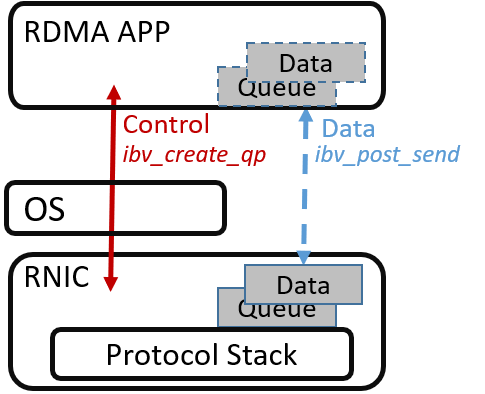
\includegraphics[width=0.8\linewidth]{images/rdma-feat.png}
	\caption{Native RDMA Architecture: the control path and data path are separated}
	\label{fig:rdma-feat}
\end{figure}

RDMA can be implemented in different ways, for example, InfiniBand~\cite{infiniband}, Roce~\cite{roce}, and iWARP~\cite{iwarp}.
OpenFabrics Enterprise Distribution (OFED \cite{ofed}) is a widely used RDMA software stack that builds an abstraction layer to hide the differences of underneath drivers and hardware.
OFED stack consists of the user-space part and the kernel-space part.
As shown in Figure~\ref{fig:rdma-feat}, in user-space, RDMA applications use Verbs APIs~\cite{verbs} to send and receive data. It is similar to socket layer for traditional network applications. On the control path, Verbs provides APIs like ibv\_create\_qp and ibv\_reg\_mr. On the data path, Verbs provides APIs like ibv\_post\_send and ibv\_post\_recv. On the control path, the Verbs library forwards requests to OFED core in OS kernel. Device specific drivers that control the RDMA hardware are registered in OFED core. On the data path, the OS kernel is bypassed. So the Verbs library calls device specific user level library to send and receive data.

In the workflow of RDMA, the control path and the data path are separated. As shown in Figure~\ref{fig:rdma-feat}, on the control path, the application explicitly creates QP~(Queue Pair), CQ~(Completed Queue), registers MR~(Memory Region) and other RDMA metadata, and caches the metadata to RNIC, such as queue ID, MR key and page tables. On the data path, the application can write to the DoorBell register to notify RNIC of a new request. RNIC will read the request in the QP, read/write the contents of the local/remote MR, and put the completion notifications into the CQ. The application can poll the CQ to get the notifications. The housekeeping work is done on the control path that involves the OS kernel. The performance critical data transmission work on the data path totally bypasses the OS kernel.
\section{Related Work} \label{relatedwork}

\textbf{Traditional TCP/IP:}\qquad TCP/IP is the basic network for each tenant in data centers. Several software solutions were proposed for traditional network virtualization. For both VMs and containers, virtual network interface cards (vRNICs) are one solution, e.g. virtio-net~\cite{virtio-russell2008}, vhost-net~\cite{vhost-net},  vhost-user-net~\cite{vhost-user-net} for VMs and veth~\cite{veth} for containers. These vRNICs are implemented in VM's or container's different space (i.e. kernel space and user space). Software-based switch, also knowed as virtual switch, in the local host brides the vNIC to physical NIC. Virtual switch can run in user space (e.g. Snabb Switch~\cite{snabb}), kernel space(e.g. Linux bridge~\cite{linux-bridge}), or both(e.g. Open vSwitch~\cite{ovs-2015}). 

\textbf{Hardware-based RDMA virtualization:}\qquad SR-IOV~\cite{sr-iov} splits a physical PCI-e device to multiple PCI-e devices, which can be allocated to VMs, providing near-native performance. In comparison to software-baed virtualization, it lacks of refficient resource management and suffers from the flexibility issue due to its virtual layer is realized in hardware. In uniRDMA, the isolation of SR-IOV are utilized and the unscalable problems are solved by dynamic vRNIC mapping. 

\textbf{Software-based RDMA virtualization:}\qquad FreeFlow~\cite{kim2019freeflow} forwards all RDMA commands from containers to the FreeFlow router (FFR) including data path. It intercepts the commands between applications and NIC drivers such as creating QP/CQ and sending/receiving data. The key different between FreeFlow and uniRDMA is that FreeFlow does capture data path commands to fitting in the container environment. Its data path commands, which accounts for the majority compared to the control path, costs extra forward latency. HyV~\cite{pfefferle2015hybrid} and MasQ~\cite{he2020masq} are designed for VMs. They achieve zero-copy and by-pass by mapping all resources. However, the implementation of memory mapping are different that is uniRDMA maps memory between virtual layer and VM's application. Moreover, HyV/MasQ backend is in kernel space while uniRDMA backend is in user space for more manageability and lightweight.
\section{Overview}

For hybrid virtual environments in clouds, RDMA virtualization not only needs to be unified, but also maintains high performance and manageability. Therefore, our design goals are as follows:

\begin{itemize}
	\item {\verb|Unification|}: Only single RDMA virtualization framework needs to be deployed in hybrid virtual environments and it provides centralized management.
	To form unified RDMA virtualization, single centralized virtual layer should be set up, which is provided to virtual machines and containers with general interfaces.
	\item {\verb|High performance|}: Performance of virtual RDMA should be close to native RDMA in terms of throughput, latency, or CPU load. Meanwhile it should suit for large-scale virtual cluster.
	\item {\verb|High manageablility|}: Basic managment shoud be meet for the clouds, such as, performance isolation, virtual network management or  portability.
\end{itemize}

% 简单介绍uniRDMA框架的工作过程
To achieve above goals, we propose a software RDMA virtualization framework, namely uniRDMA. As Figure~\ref{fig:framework-overview} shows, uniRDMA consists of vRNICs(including its' driver/library in VMs or containers) and the virtual layer:

vRNICs is a simple software emulation of physical RNIC. Each vRNIC is instanced in the virtual layer when VM or container's RDMA applications start. The RDMA commands of applications can be transported to vRNIC through guest driver or container libraries. Besides, RDMA resources (e.g. QPs and DoorBells) in vRNICs are mapped to physical RNIC and upper applications. Thus, the data commands in application can be executed locally for high-performance.

The virtual layer is also in host user space. We design it for centralized management of vRNICs. It controls all RDMA devices through RDMA verbs library in host user space. Meanwhile, vRNICs are configured in the virtual layer to construct virtual RDMA network, e.g. vRNIC addresses and routing rules.

\begin{figure}[!ht]
	\centering
	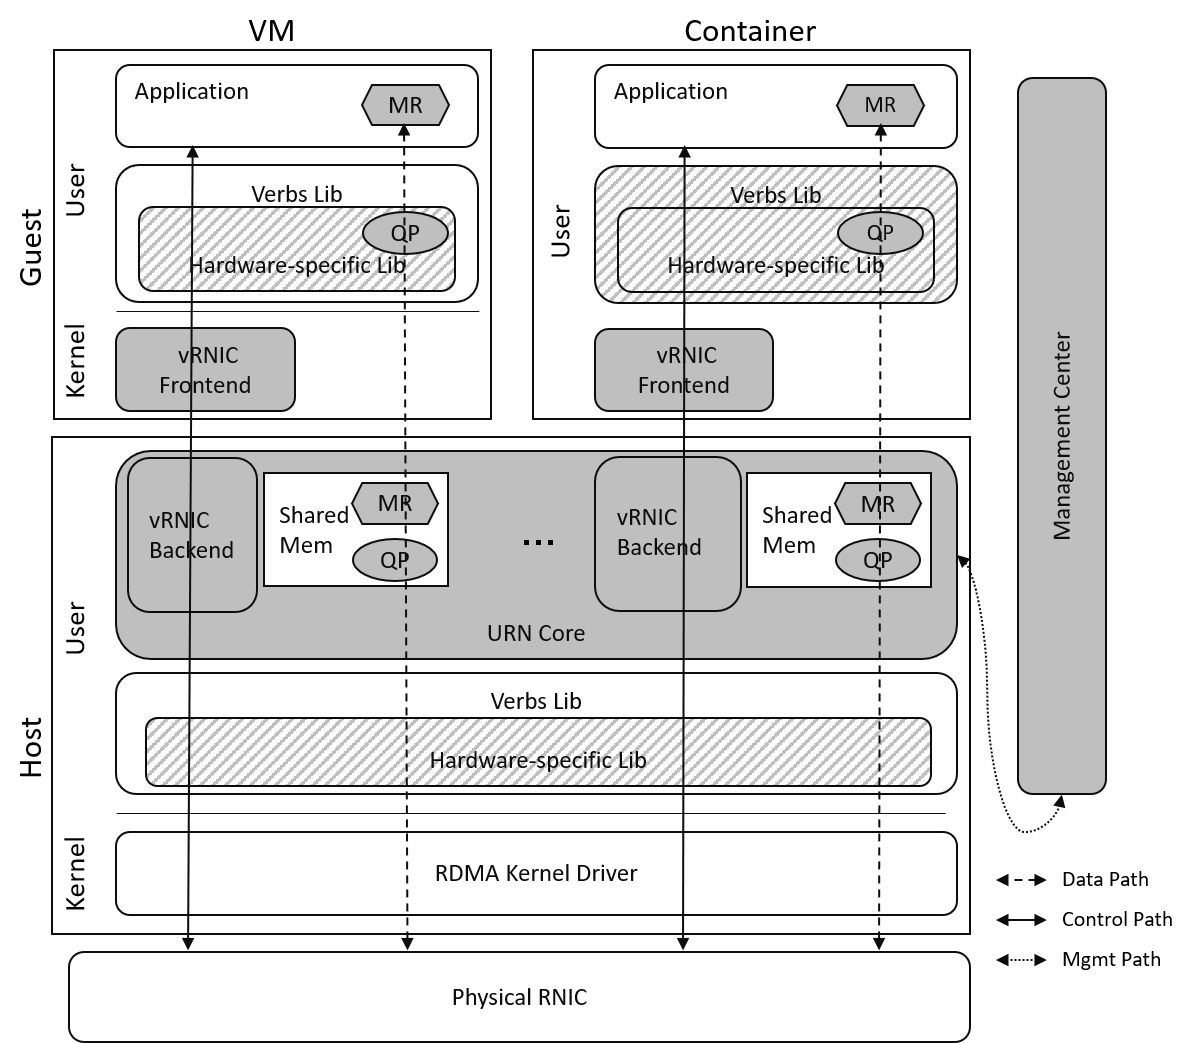
\includegraphics[width=0.9\linewidth]{images/framework-overview.png}
	\caption{uniRDMA Framework Overview}
	\label{fig:framework-overview}
\end{figure}


\section{Unified Virtual Layer}
 The main work of uniRDMA virtual layer is including vRNIC virtualization, vRNIC mapping  and virtual RDMA network management.The primary challenges are to make both isoaleted and high-performance for different vRNICs in the same virtual layer. 
	
\subsection{vRNIC Virtualization}
The first problem is which space the virtual layer(including vRNICs) is located: kernel space or user space. Because container applications and virtual machines are both host processes, they can interact with the host kernel or other host processes. In addition, there are both user-level and kernel-level RNIC interface. Therefore, both kernel space and user space can realize the unified RDMA virtual layer. However, user space layer is friendly to containers because of lightweight and in favour of secure and flexible management. Moreover, software development in user space is less difficult, more portable and compatible. Therefore, uniRDMA chooses a user space virtual layer.

The RDMA resources is the key in both control path and data path at RDMA communication. In control path, the application creates queue instances such as QP, and registers memory regions(MRs) in host memory; In data path, the application writes DoorBell to notify RNIC to deal with WQE in QP and transform data in MRs.So, vRNIC virtulization is mainly about how to construct the virtual RDMA resoucrs to provide complete RDMA communication. We summarize that RNIC has two kinds of hardware properties about theses RDMA resources, namely static property and dynamic property:

For static properties,  since RDMA sends and receives messages based on QPs, MRs and other RDMA resources, it can be abstracted that the RDMA NIC has the following buffers inside:

\begin{itemize}
\item {\verb|Queue Buffer|}: storing information of queue instances, such as QP number, QP state and CQ number. The network card uses the information to read and write work requests, establish connections with remote QPs, etc.  
\item {\verb|Data Buffer|}: storing the information of registered memory regions, such as page table, memory key, etc. The network card use the informaation to access local or remote memory for data transform.  
\item {\verb|Doorbell Buffer|}: including multiple doorbell registers. The network card use it to accept user commands and notify the internal hardware processor to perform DMA, processing and forwarding. 
\end{itemize}

For dynamic attributes, Therefore, the state of RDMA resources are daynamic in control path and data path. Control path includes the creation and destruction of RDMA resources. RDMA resources or informations in buffer are always changed.For example, RNIC records the QP number when QP is created, changes QP state for RDMA connection and clear QP informations in the destory. Nofity that this porcess has losts latency due to the kernel, Data path is mainly about the usage of RDMA resources.RDMA resources or informations in buffer are always maintained in RNIC. When RDMA applications post a send or receive operation, only write the DoorBell and the hardware processor performs DMA, encapsulates and forwards data.

To emulate the static attributes, virtual queue, data and doorbell buffers are respectively set up in vRNIC. For example, the QP buffer stores virtual QP information and the virtual doorbell buffer is include virtual doorbells. Virtual buffer is flexible and unlimited for the nums of RDMA resoucrs instances. 

To emulate the dynamic attributes, apparently, if only using pure software, it may cause low performance because of the software overhead in whole RDMA communication. Fortunately, we found all RDMA reources informations in RNIC are only changed in control path and maintained in data path. So, we can map the virtual RDMA reources to RNIC only in control path, such as QP and Doorbell,  and do not need introduce any operations in data path. Mapped RDMA resources are directly used and RNIC is notified by mapped virtual DoorBell in vRNIC. As a result, vRNIC are still with DMA zero-copy, hardware protocol stack processing and other high-performance capability in data path. Therefore, we put each vRNIC with with a map unit. As Figure~\ref{fig:map-unit} shows, it maps or unmaps virtual RDMA resources from vRNIC to RNIC in control path:

\begin{figure}[!ht]
	\centering
	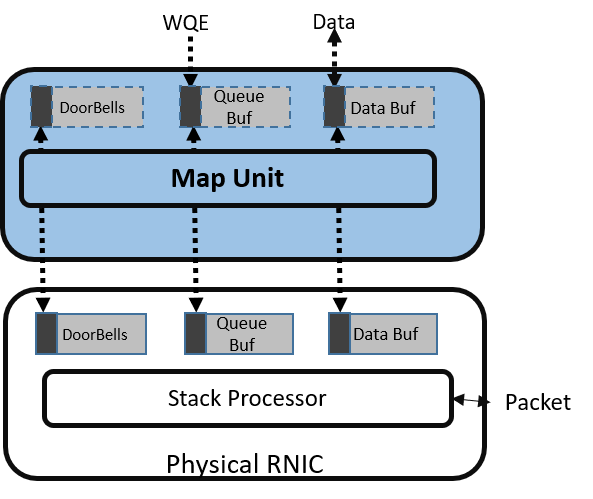
\includegraphics[width=1.0\linewidth]{images/map-unit}
	\caption{Map Unit in vRNIC}
	\label{fig:map-unit}
\end{figure}

For RDMA resources(e.g. QPs, CQs): Taking QP as an example, regularly, vRNIC record virtual RDMA resources informations when the virtual QP instance are created. However, virtual QP are still not generated-associated with the RNIC. To make the maping, the map unit will create corresponding real QP instance in RNIC based on the information of virtual QP instances, such as the same memory address information and the same device id. Equivalently, the virtual QP informations are recongnized in RNIC, such as QP number and QP state, and can be one-to-one synchronous with RNIC's  physical instance by lots of similar map operations in control path. All operations can be completed by calling the Verbs interface of RNIC in user space. After the mapping is completed, the work requests in the vRNIC virtual QP can be zero-copied into the RNIC. Also, data in registered memroy of vRNIC can also be zero-copied to RNIC in the same way. 

For DoorBells: It needs to be mapped to the hardware doorbell in the physical NIC device space, so that vRNIC has the ability to notify the RNIC hardware processors. In vRNIC, the mapping unit will map the virtual address of the virtual doorbell to the hardware doorbell address of the corresponding physical NIC device space through a system call. As shown in Figure 4-2, after the mapping is completed, the write operation to the vRNIC virtual doorbell is equivalent to performing the doorbell notification to the RNIC.

Map unit is the key for vRNICs' performance.Note that all mapping relationships are all one-to-one, therefore, the correctness and isolation of resources in different RDMA context are guaranteed. Meanwhile, because the mapping operation is only executed in control path, the overhead are one-off compared to data commands. For the data path, vRNICs can directly utilize the hardware processing capability of RNIC, such as DMA zero-copy and hardware protocol stack processing.

\subsection{vRNIC Mapping}
The same virtual layer needs to create multiple vRNICs and provide them to different containers or virtual machines respectively. If each vRNIC is directly mapped to the same RNIC, it will compete for the same PCIe bus and share the configuration space of RNIC. The vRNICs are still not isolated or limited.

SR-IOV is a popular hardware-based virtualization technology.RNIC can virtualize multiple different hardware interface, called VFs. Each VF has an unique PCIe bus and configuration space. At the same time, when configuring VFs, users can limit network rate and other hardware resources, and implement management policies such as QoS. The uniRDMA virtual layer maps each vRNIC to the VF interface of RNIC separately, so hardware-level isolation are guaranteed for vRNICs.

However, the VF resources of SR-IOV are limited, for example, only 126 VFs are supported in Mellanox ConnectX-3 at most~\cite{ofed-manual}. Therefore, the existing VFs need to be managed and coordinated in a unified to meet many vRNICs.

\begin{figure}[!ht]
	\centering
	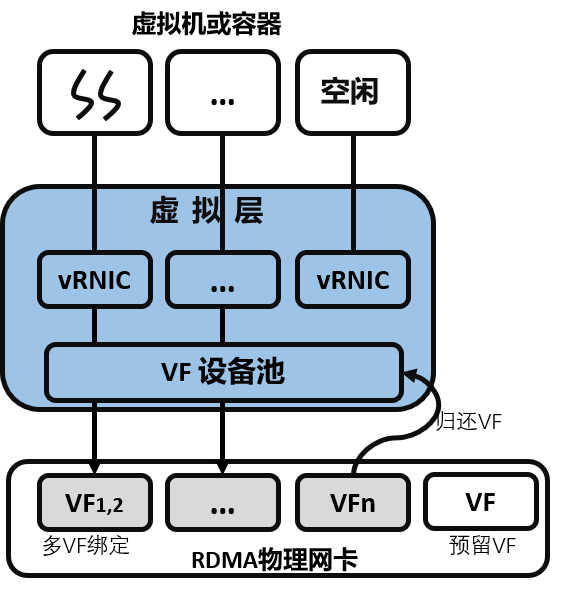
\includegraphics[width=1.0\linewidth]{images/vf-mapping}
	\caption{Management of vRNIC Mapping}
	\label{fig:vf-mapping}
\end{figure}

As Figure~\ref{fig:vf-mapping} shows: First, the virtual layer constructs a dynamic VF pool. The initial number of VFs in the pool is usually the number of pre-determined virtual instances. If lack of free VFs in the pool, the device pool can dynamically expand the number of VFs. Second, the virtual layer supports dynamic mapping between vRNIC and VF. When all virtual RDMA resources have been destroyed, the virtual layer marks the VF as idle and puts it back into the pool. So thatt the virtual layer can support the number of vRNICs that exceed the VF limit. Finally, the virtual layer supports various mapping relationships between vRNICs and VFs. For example, load balancing can be meeted by map a vRNIC with multipe VFs. VF resources are saved by mapping multiple vRNICs of the same virtual instance to the single VF. 

\subsection{Virtual RDMA Management}
To maintain portability and realize RDMA network management, RDMA connections between vRNICs can not be established by the physical address of VFs. But this problem has a solution that uniRDMA virtual layer acts as a software RDMA switch or router for virtual RDMA network configuration and routing management, etc.

RNICs are usually managed by the subnet manager in the cluster. For the same purpose, a control center is set up in uniRDMA to assign virtual RDMA addresses vGIDs to each vRNIC and configure routing rules between vRNICs. As shown in Figure~\ref{fig:route-config} , the vRNICs are divided into two groups: group 1 and group 2; vRNICs in the same group are allowed to establish RDMA connections, and cross-group RDMA connections can not succeed due to the isolated routing rules between group 1 and group 2.

\begin{figure}[!ht]
	\centering
	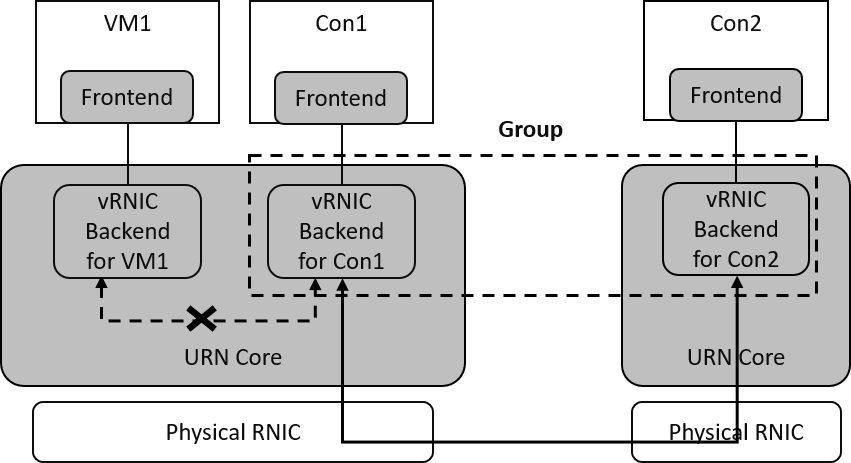
\includegraphics[width=1.0\linewidth]{images/route-config}
	\caption{Virtual RDMA Network Routing}
	\label{fig:route-config}
\end{figure}

Consistent with native RDMA, vRNICs in each virtual layer need to exchange each other's virtual RDMA addresses, virtual QP queue information, registered memory keys and other information to establish virtual RDMA connections. However, the vRNIC RDMA address is virtual, and does not recognized in RNIC. Therefore, the mapping relations between the virtual addresses of vRNICs and the physical addresses of VF needs to be exchanged between virtual layers. When establishing the virtual RDMA connection, the virtual RDMA address is converted to the physical address of the mapped VFs. Note that RDMA resources informations, such as virtual QP number and memory keys, have been mapped to the VF interface by the map unit in vRNIC, they can all be recognized VF and directly used to create RDMA connection.


\section{General vRNIC interface}
In native RDMA, the application accesses RNIC by the Verbs interface. Correspondingly, we presents uniVerbs interface, which is general to containers and virtual machines. Moreover, the interfaces have strong isolation and are transparent to all RDMA applications. At the same time, uniVerbs interface maps RDMA resources bewteen RDMA applications and vRNICs for zero copy and bypassing the virtual layer.
	
\subsection{Basic uniVerbs Interface Construction}
The RDMA applications in containers and virtual machines are both the processes of host. Therefore, the general interface are avialable for both containers and virtual machines. 

For containers, vRNIC can be directly provided to RDMA applications in containers by IPC(inter-process communication). However, for virtual machines, the vRNIC in the host user space and the RDMA application in the virtual machine user space are separated from the emualted hardware environment and the guest operating system. Therefore, it is necessary to use I/O virtualization technology to extend each vRNIC as an I/O device of the virtual machine. Then, driver for this device must be installed in virtual machine to support the I/O process. Therefore, the uniVerbs interface for the virtual machine includes two following works:

\begin{itemize}
\item {\verb|Extend vRNIC as I/O device|}: 
The existing I/O virtualization technologies are mainly divided into full virtualization and paravirtualization. The full virtualization completely simulates all the functions of the device, there are frequent context switching and data copy overhead. 
In contrast, paravirtualization does not emulate the hardware complemently to reduce the times of data copy and switch. Therefore, we exploit paravirtualization to expand vRNIC as an I/O device. In our design, the I/O channel between vRNIC and the virtual machine is a shared memory queue, which is created by file; the signal and interrupt mechanism can be realized through the event descriptor between virtual layer process and each virtual machine process, then the event notification is converted into an internal interrupt signal by virtual machine monitor.
 
\begin{figure}[!ht]
	\centering
	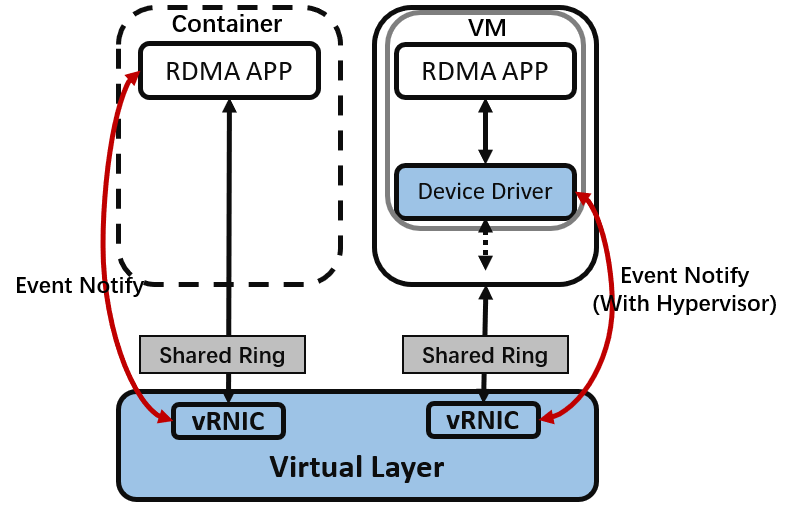
\includegraphics[width=1.0\linewidth]{images/interface-general}
	\caption{General uniVerbs Interface}
	\label{fig:interface-general}
\end{figure}


\item {\verb|Design the I/O device driver|}:
The goal of the device driver is to support I/O process inside each guest. As shown in in Figure~\ref{fig:interface-general},  the commands of RDMA application be forwared into the memory-shared queue, and trigger events to notify the vRNIC to process them; similarly, the device driver receives interrupt notifications and reads the result from vRNIC. In short, the device driver can be implemented by a lightweight kernel module.

\end{itemize}

 For generality, As shown in in Figure~\ref{fig:interface-general}, the same design as virtual machines is adopted for containers: in I/O channel, the file-based shared queue is also used; in the synchronization mechanism, the same event notification mechanism is used. But remind the container does not fall into the monitor or inject interrupts during the synchronization.

When there are multiple virtual machines or containers, if the files of each vRNIC are not isolated, they can be discovered by every container through scanning files. In order to solve this problem, we runs the virtual machine in a isolated container environment. Based on the container's mount namespace, we respectively place the shared files of each vRNIC in the dedicated directories and mounts each directory to the corresponding container(including containers running virtual machines). As a result, due to the isolation of the mount namespace, the shared files of each vRNIC in the virtualization layer are only visible to the used container or virtual machine.  

\begin{figure}[!ht]
	\centering
	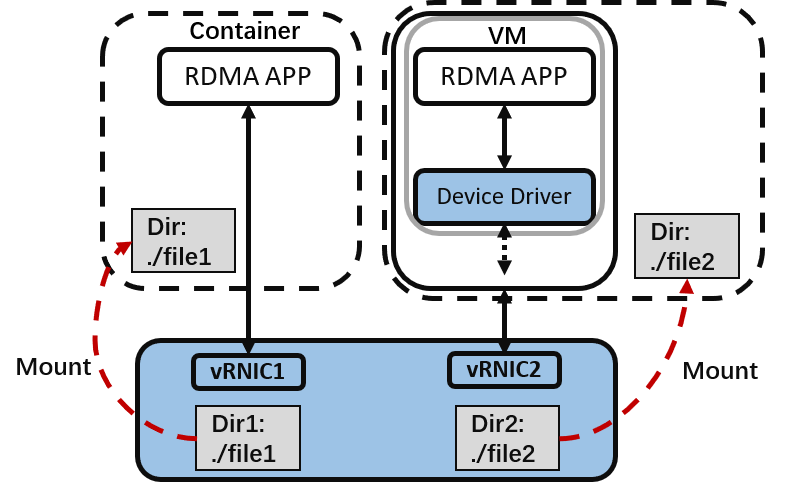
\includegraphics[width=1.0\linewidth]{images/interface-isolate}
	\caption{General uniVerbs Interface}
	\label{fig:interface-isolate}
\end{figure}

\subsection{uniVerbs Interface Optimization}
After completing the interface construction, the requests of RDMA applications can be transmitted to vRNICs, and the results can also be returned to the applications. In uniVerbs, zero copy of data and bypassing the virtual layer are realized by mapping the RDMA resources to vRNIC. As a result, data commands do not need to be forward to the virtual layer and this mode is consistent with native RDMA.

(1) zero copy optimization
The zero copy contents are including the RDMA work request in the QP queue and the transfer data in the registered memory, and the process is from RDMA application to pyhiscal RNIC. Remind that vRNIC RDMA resources are mapped to VFs, so we only need to make sure the zero-copy from RDMA application to vRNIC.

The fact of zero-copy is that both processes have common availiable physical memory pages. Similar as the above I/O channels, file-based shared memory are also used when mapping QP and other RDMA resouces and this is general for both virtual machines and containers.

\begin{figure}[!ht]
	\centering
	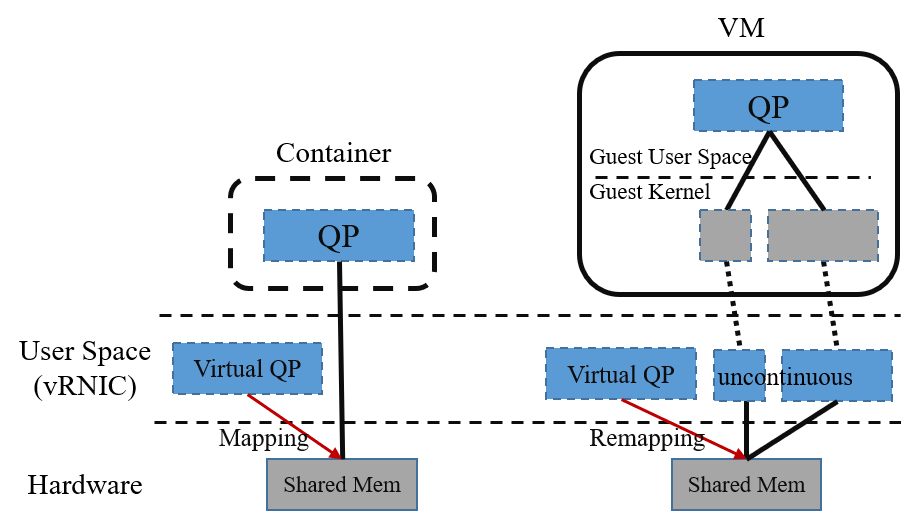
\includegraphics[width=1.0\linewidth]{images/zero-copy}
	\caption{Mapping QP to vRNIC}
	\label{fig:zero-copy}
\end{figure}

However, in the virtual machine, due to the memory management mechanism of guest operating system, the virtual machine's physical memory of the RDMA resource may be not continuous, and the mapped memory area in vRNIC is not continuous. So, vRNIC can not map the virtual memory area as a virtual RDMA resource to RNIC. To solve this problem, the virtual memory remapping mechanism in user space is used. It remaps the discontinuous RDMA resource virtual memory area in vRNIC to the a block of continuous virtual memory, and the  sequence of mapped physical memory page must be unchanged.

(2) Bypassing virtual layer optimization
Pressing the doorbell is necessary in RDMA data path to drive RNIC. In vRNIC, the doorbell that is mapped to VF, still need to be mapped to RDMA application tp meet bypassing. Otherwise, the pressing command needs be forward to vRNIC and thats imports apperant latency in data path.

However, the RDMA application and the vRNIC belong to two different processes on the host, and they have isolated virtual address spaces. At the same time, the doorbell register is located in the device address space and cannot be mapped by shared memory. The key to solving this problem is that the process of RDMA application needs to know the physical address of the doorbell register.

\begin{figure}[!ht]
	\centering
	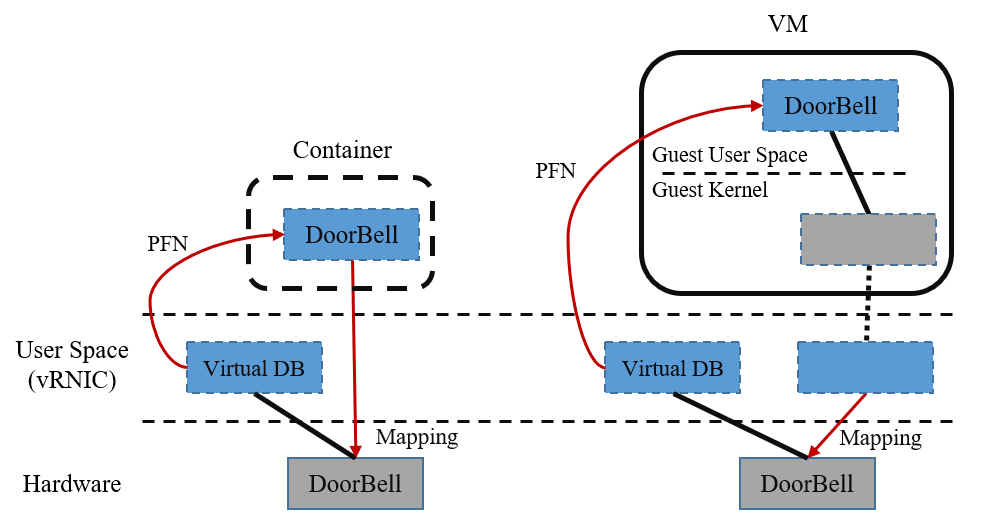
\includegraphics[width=1.0\linewidth]{images/by-pass}
	\caption{Mapping DB from vRNIC}
	\label{fig:by-pass}
\end{figure}

Therefore, when an RDMA application creates a RDMA context, it sends a request to the vRNIC at first. Under the supervision of virtual layer, vRNIC forwared to application with the corresponding physical address of the doorbell, commonly the physical page number. After that, the application maps its doorbell virtual address to the physical page in its own process, that needs the host kernel and hypervisor if the application in virtual machines.


\section{Evaluation} \label{eval}
In this section, we evaluate the performance of \sys based on the RDMA test tools and real applications. We expect to answer the following questions:

\begin{itemize}
\item How about the performance of \sys compared to that of native RDMA for both VMs and containers?
\item Can \sys be adapted to the real-world RDMA applications in both VMs or containers?
\end{itemize}

\subsection{Experiment Methodology}
All experiments are carried out on two servers. The settings mainly include three parts: host server, container and virtual machine. 

Each host server is equipped with 4 Intel Xeon E7-4850 2.40GHz 16-core CPUs and 1 TB RAM. The RNIC used is Mellanox ConnectX-3 56 Gb/sec, which performs RDMA communication under Infiniband.  The operating system is CentOS 7.4.1708 (Linux 3.10.0-693.el7.x86\_64). The RDMA driver installed on the host server is Mellanox OFED 4.4-2.0.7.0~\cite{mlnx-ofed}. To keep the consistence, VMs and containers are built based on the same OS images as host. All virtual machines are based on QEMU(5.1.50)~\cite{qemu} enabled with KVM~\cite{kvm}. We provide 16 cores and 64 GB memory for each VM. We run containers using Docker(18.06.1-ce)~\cite{docker} and limit the CPU and memory resources to the same settings as the VM. In addition, all the applications are compiled with GCC/G++ 4.8.5 with the O3 compilation configuration. 


\subsection{Basic benchmark}
Throughput and latency are the key target of network performance. RDMA supports two different data transmission modes: one-sided and two-sided. Due to the difference performance between them, we evaluate them respectively.

Based on the RDMA benchmark test tool perftest~\cite{perftest}, we evaluated the throughput and latency of \sys, native RDMA, hardware virtualization SR-IOV, and software virtualization FreeFlow in virtual machines or containers. For two-sided operations (Send and Recv), we use the ``ib\_send\_bw'' and ``ib\_send\_lat'' commands; for one-sided operations (Write and Read), with Write as the representative, we use the ``ib\_write\_bw'' and ``ib\_write\_lat'' commands. The specific process is: after the RDMA connection is established between the client and the server, the bytes of transmitted message each time will be increased from 4B to 1MB, the data will be iteratively transmitted 1000 times with each message size, and finally the average throughput and latency are calculated.

(1) Throughput: The results of two-sided operation are shown in Figure~\ref{fig:send-bw}, and the one of one-sided operation are shown in Figure~\ref{fig:write-bw}. Whether \sys is in a virtual machine or in a container scenario, the throughput of its two-sided and one-sided operations is similar as SR-IOV and close to native RDMA.

Compared with FreeFlow, when the message is small, the throughput of \sys has reached 4-6 times that of FreeFlow. Because FreeFlow forwards all data commands to the software virtualization layer for processing. Therefore, the forward latency gradually accumulates and decrease the throughput significantly. However, \sys maps all RDMA resources to execute data commands in the user space of the container or virtual machine. Therefore, there is no latency for commands forwarding in data path.

\begin{figure}[!ht]
	\centering
	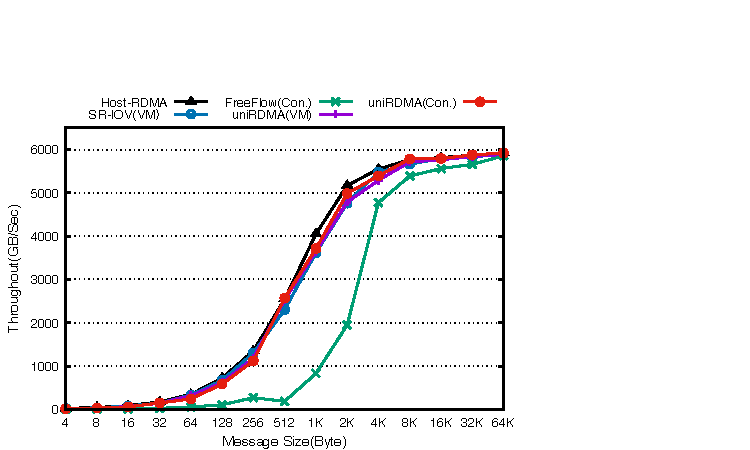
\includegraphics[width=1.0\linewidth]{images/send-bw.pdf}
	\caption{The Throughout of RDMA Send and Recv}
	\label{fig:send-bw}
\end{figure}

\begin{figure}[!ht]
	\centering
	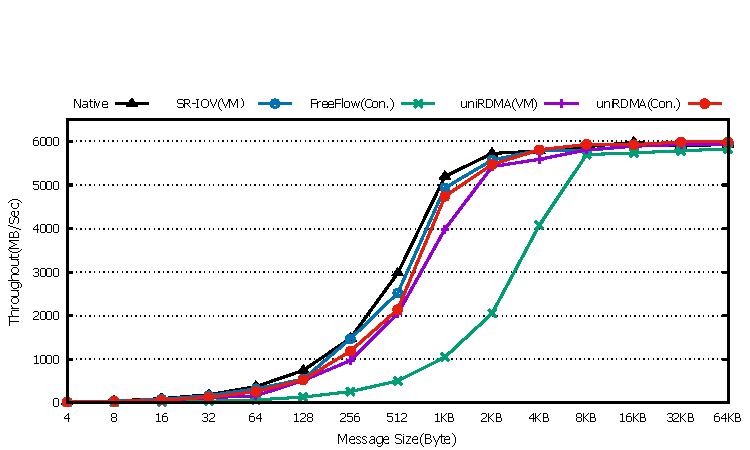
\includegraphics[width=1.0\linewidth]{images/write-bw.pdf}
	\caption{The Throughout of RDMA Write}
	\label{fig:write-bw}
\end{figure}

When the message gradually increases, such as reaching 64KB, the throughput of each framework tends to be consistent. The reason is that the bandwidth is saturated, and the delay overhead of FreeFlow has been covered by waiting delay in RNIC.

(2) Latency: The results of two-sided operation are shown in Figure~\ref{fig:send-lat}, and the one of one-sided operation are shown in Figure~\ref{fig:write-lat}. Whether \sys is in a virtual machine or in a container scenario, the latency of its two-sided and one-sided operations is similar as SR-IOV and close to native RDMA.

Compared with FreeFlow, when the message is small, the latency of \sys has reached 40\%~60\% of FreeFlow because of FreeFlow's forwarding latency. Also, when the message gradually increases, such as reaching 64KB, the latency of each framework tends to be consistent. Because the main latency has been caused by RNIC data processing.

\begin{figure}[!ht]
	\centering
	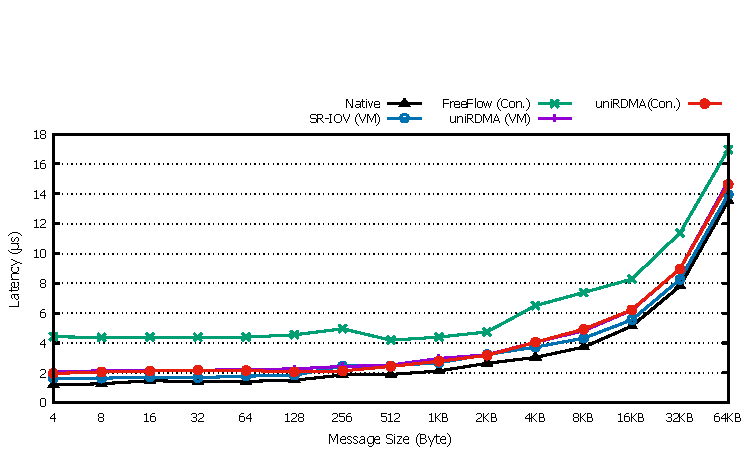
\includegraphics[width=1.0\linewidth]{images/send-lat.pdf}
	\caption{The Latency of RDMA Send and Recv}
	\label{fig:send-lat}
\end{figure}

\begin{figure}[!ht]
	\centering
	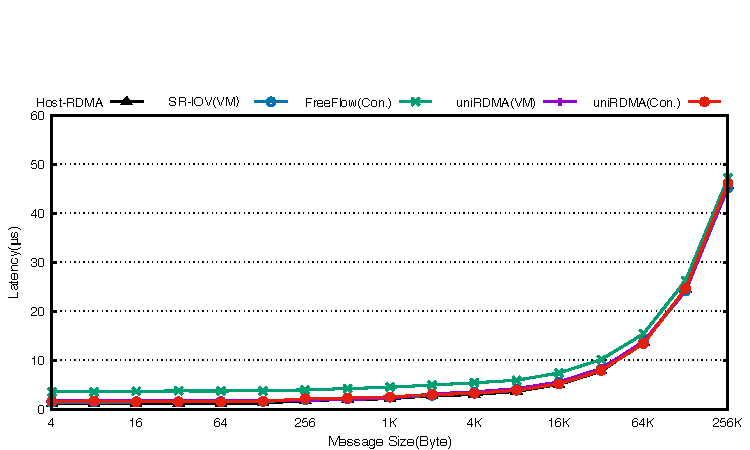
\includegraphics[width=1.0\linewidth]{images/write-lat.pdf}
	\caption{The Latencty of RDMA Write}
	\label{fig:write-lat}
\end{figure}

\subsection{Real-world Applications}

The worth of RDMA is mainly about its optimized performance in real-world applications. RDMA virtualization needs to maintain the performance close to native RDMA. Therefore, we evaluate \sys and other frameworks in high-performance computing benchmark Graph-500. Graph-500 is a benchmark framework used to test the performance of the Message Passing Interface (MPI). Based on the constructed graph structure, users test the performance of breadth-first search (BFS) and single source shortest path (SSSP). The performance index is the number of edges traversed per second (traversed edges). per second, TEPS), the larger the value, the better the performance.

In this paper, the node scale of the computational graph in Graph-500 is set to 26, and the ratio of edges to points is set to the default parameter of 16. The constructed graph has a total of 2$^{25}$ vertices, with 2$^{29}$ edges, the entire graph occupies approximately around 16GB. When testing BFS and SSP, 16 MPI processes are scattered and executed on two nodes in turn, and the average value is taken according to the results of 12 tests. The data obtained is shown in Table Figure~\ref{fig:graph-500} (because there are core dump problems when using FreeFlow for Graph-500, the corresponding data is lacking).

As shown in Figure~\ref{fig:graph-500},  the performance of \sys is close to native RDMA. Because \sys bypasses the kernel and virtualization layer in the data path, and there is no forwarding latency.

\begin{figure}[!ht]
	\centering
	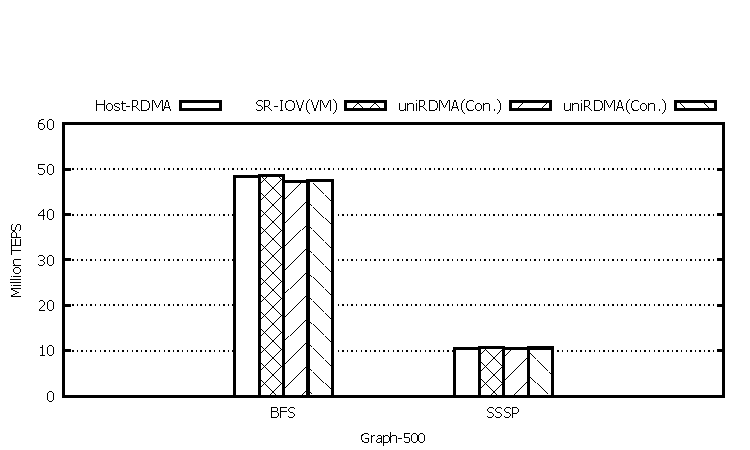
\includegraphics[width=1.0\linewidth]{images/graph-500.pdf}
	\caption{The Performance of Graph-500}
	\label{fig:graph-500}
\end{figure}
\section{Discussion}
In this section, there are some concerns about uniRDMA in cloud environments:
\begin{itemize}
	\item {\verb|Security|}: uniRDMA's virtual layer is in the user space. Unlike HyV and MasQ, RDMA resources, including data, do not need to be mapped to the kernel space. Therefore, it avoids buffer overflow and other attacks against the kernel. Through the isolated vRNIC and interface, there are no potential threats between different virtual instances.
	\item {\verb|Other network extensions|}: The high performance of RDMA can integrate other network protocol stacks, such as TCP/IP networks, to optimize the performance of network applications. Existing work includes vSocket and so on~\cite{wang2019vsocket}~\cite{li2019socksdirect}. However, there is currently no unified RDMA-based optimized socket for container and virtual machine applications, and uniRDMA can be also easily extended to meet it.
	\item {\verb|Virtual Instances Migration|}: For virtual instances containing RDMA applications, uniRDMA can directly migrate statically without reconfiguring the RDMA address, etc., only for dynamic migration in the virtual, because RDMA bypasses the transmission mechanism of the kernel and remote read and write, its memory capacity It is difficult to perceive management and monitoring, and uniRDMA needs to cooperate with other research work to achieve this goal~\cite{firestone2018accelnsdi}.
\end{itemize}


\section{Conclusion}
In this paper, we design a unified RDMA virtualization framework, namely uniRDMA, which consists of single user-space virtual layer and general uniVerbs interfaces. In the user space virtual layer: the isolated and high-performance vRNICs are virtualized based on the VFs from SR-IOV; In the uniVerbs interfaces: uniRDMA uses shared files to realize general I/O channel for VMs and containers; the isolation of interface is ensured with mount namespace in containers; uniVebrs realizes zero-copy and bypassing virtual layer in RDMA data path, by mapping all RDMA resource between vRNIC and RDMA applications. The experimental results show that uniRDMA has high performance close to native RDMA while meeting generality and management.





%%
%% The next two lines define the bibliography style to be used, and
%% the bibliography file.
\bibliographystyle{ACM-Reference-Format}
\bibliography{reference}

%%
%% If your work has an appendix, this is the place to put it.
%\appendix



\end{document}
\endinput
%%
%% End of file `sample-sigconf.tex'.
